\scnsegmentheader{Предметная область и онтология субъектно-объектных спецификаций воздействий}
\begin{scnsubstruct}
    \begin{scnrelfromlist}{соавтор}
        \scnitem{Гордей А.Н.}
        \scnitem{Никифоров С.А.}
        \scnitem{Бобёр Е.С.}
        \scnitem{Святощик М.И.}
    \end{scnrelfromlist}
    \scniselement{предметная область и онтология}
    \scnheader{индивид}
    \scnidtftext{часто используемый sc-идентификатор}{субъект}
    \scnrelfrom{источник}{\cite{Hardzei2005}}
    \scnheader{участник воздействия\scnrolesign}
    \scnidtf{участник акции\scnrolesign}
    \scniselement{ролевое отношение}
    \scnrelfrom{первый домен}{индивид}
    \scnrelfrom{второй домен}{воздействие}
    \scntext{explanation}{\textit{участник акции\scnrolesign} -- это ролевое отношение, которое связывает акцию с участвующим в ней индивидом.}
    \scnrelfrom{источник}{\cite{Hardzei2021}}
    \scnrelfrom{источник}{\cite{Fillmore1977}}
    \scnrelfrom{источник}{\cite{Fillmore1982}}
    \begin{scnsubdividing}
        \scnitem{субъект\scnrolesign
            ~\\\scntext{explanation}{\textit{субъект\scnrolesign} -- инициатор акции.}
            \begin{scnsubdividing}
                \scnitem{инициатор\scnrolesign
                    ~\\}
                \scnitem{вдохновитель\scnrolesign
                    ~\\}
                \scnitem{распространитель\scnrolesign
                    ~\\}
                \scnitem{вершитель\scnrolesign
                    ~\\\scntext{explanation}{\textit{вершитель\scnrolesign} завершает акцию производством из объекта продукта.}}
            \end{scnsubdividing}
        }
        \scnitem{инструмент\scnrolesign
            ~\\\scntext{explanation}{\textit{инструмент\scnrolesign} -- исполнитель акции.}
            \begin{scnsubdividing}
                \scnitem{активатор\scnrolesign
                    ~\\\scntext{explanation}{\textit{активатор\scnrolesign} непосредственно воздействует на медиатор.}}
                \scnitem{супрессор\scnrolesign
                    ~\\\scntext{explanation}{\textit{супрессор\scnrolesign} подавляет сопротивление медиатора.}}
                \scnitem{усилитель\scnrolesign
                    ~\\\scntext{explanation}{\textit{усилитель\scnrolesign} наращивает воздействие на медиатор.}}
                \scnitem{преобразователь\scnrolesign
                    ~\\\scntext{explanation}{\textit{преобразователь\scnrolesign} преобразует медиатор в инструмент.}}
            \end{scnsubdividing}
        }
        \scnitem{медиатор\scnrolesign
            ~\\\scntext{explanation}{\textit{медиатор\scnrolesign} -- посредник акции.}
            \begin{scnsubdividing}
                \scnitem{ориентир\scnrolesign
                    ~\\}
                \scnitem{локус\scnrolesign
                    ~\\\scntext{explanation}{\textit{локус\scnrolesign} частично или полностью окружает объект и тем самым локализует его в пространстве.}}
                \scnitem{транспортёр\scnrolesign
                    ~\\\scntext{explanation}{\textit{транспортёр\scnrolesign} перемещает объект.}}
                \scnitem{адаптер\scnrolesign
                    ~\\\scntext{explanation}{\textit{адаптер\scnrolesign} приспосабливает  инструмент к воздействию на объект.}}
                \scnitem{материал\scnrolesign
                    ~\\\scntext{explanation}{\textit{материал\scnrolesign} используется в качестве объекта-сырья для производства продукта.}}
                \scnitem{макет\scnrolesign
                    ~\\\scntext{explanation}{\textit{макет\scnrolesign} является исходным образцом для производства из объекта продукта.}}
                \scnitem{фиксатор\scnrolesign
                    ~\\\scntext{explanation}{\textit{фиксатор\scnrolesign} превращает переменный локус объекта в постоянный.}}
                \scnitem{ресурс\scnrolesign
                    ~\\\scntext{explanation}{\textit{ресурс\scnrolesign} питает инструмент.}}
                \scnitem{стимул\scnrolesign
                    ~\\\scntext{explanation}{\textit{стимул\scnrolesign} проявляет параметр объекта.}}
                \scnitem{регулятор\scnrolesign
                    ~\\\scntext{explanation}{\textit{регулятор\scnrolesign} служит инструкцией в производстве из объекта продукта.}}
                \scnitem{хронотоп\scnrolesign
                    ~\\\scntext{explanation}{\textit{хронотоп\scnrolesign} локализует объект во времени.}}
                \scnitem{источник\scnrolesign
                    ~\\\scntext{explanation}{\textit{источник\scnrolesign} обеспечивает инструкциями инструмент.}}
                \scnitem{индикатор\scnrolesign
                    ~\\\scntext{explanation}{\textit{индикатор\scnrolesign} отображает параметр воздействия на объект или параметр продукта как результата воздействия на объект.}}
            \end{scnsubdividing}
        }
        \scnitem{объект\scnrolesign
            ~\\\scntext{explanation}{\textit{объект\scnrolesign} -- реципиент акции.}
            \begin{scnsubdividing}
                \scnitem{покрытие\scnrolesign
                    ~\\\scntext{explanation}{\textit{покрытие\scnrolesign} -- внешняя изоляция оболочки индивида.}}
                \scnitem{корпус\scnrolesign
                    ~\\\scntext{explanation}{\textit{корпус\scnrolesign} -- оболочка индивида.}}
                \scnitem{прослойка\scnrolesign
                    ~\\\scntext{explanation}{\textit{прослойка\scnrolesign} -- внутренняя изоляция оболочки индивида.}}
                \scnitem{сердцевина\scnrolesign
                    ~\\\scntext{explanation}{\textit{сердцевина\scnrolesign} -- ядро индивида.}}
            \end{scnsubdividing}
        }
        \scnitem{продукт\scnrolesign
            ~\\\scntext{explanation}{\textit{продукт\scnrolesign} -- результат воздействия субъекта на объект.}
            \begin{scnsubdividing}
                \scnitem{заготовка\scnrolesign
                    ~\\\scntext{explanation}{\textit{заготовка\scnrolesign} -- превращённый в сырьё объект.}}
                \scnitem{полуфабрикат\scnrolesign
                    ~\\\scntext{explanation}{\textit{полуфабрикат\scnrolesign} -- наполовину изготовленный из сырья продукт.}}
                \scnitem{прототип\scnrolesign
                    ~\\\scntext{explanation}{\textit{прототип\scnrolesign} -- опытный образец продукта.}}
                \scnitem{изделие\scnrolesign
                    ~\\\scntext{explanation}{\textit{изделие\scnrolesign} -- готовый продукт.}}
            \end{scnsubdividing}
        }
    \end{scnsubdividing}
    \scnheader{воздействие}
    \scnidtf{акция}
    \scnrelfrom{источник}{\cite{Hardzei2017}}
    \scnrelfrom{разбиение}{\scnkeyword{Типология по характеру взаимодействия участников\scnsupergroupsign}
    }
    \begin{scneqtoset}
        \scnitem{воздействие активизации
            ~\\\scntext{explanation}{\textit{воздействие активизации} -- воздействие, в ходе которого взаимодействие осуществляется между субъектом и инструментом.}}
        \scnitem{воздействие эксплуатации
            ~\\\scntext{explanation}{\textit{воздействие эксплуатации} -- воздействие, в ходе которого взаимодействие осуществляется между инструментом и медиатором.}}
        \scnitem{воздействие трансформации
            ~\\\scntext{explanation}{\textit{воздействие трансформации} -- воздействие, в ходе которого взаимодействие осуществляется между объектом и продуктом.}}
        \scnitem{воздействие нормализации
            ~\\\scntext{explanation}{\textit{воздействие нормализации} -- воздействие, в ходе которого взаимодействие осуществляется между объектом и продуктом.}}
    \end{scneqtoset}
    \scnrelfrom{разбиение}{\scnkeyword{Типология воздействий по виду взаимодействующих подсистем\scnsupergroupsign}
    }
    \begin{scneqtoset}
        \scnitem{воздействие среда-оболочка
            ~\\}
        \scnitem{воздействие оболочка-ядро
            ~\\}
        \scnitem{воздействие ядро-оболочка
            ~\\}
        \scnitem{воздействие оболочка-среда}
    \end{scneqtoset}
    \scnheader{воздействие}
    \scnrelfrom{разбиение}{\scnkeyword{Типология воздействий по фазам наращивания воздействия\scnsupergroupsign}
    }
    \begin{scneqtoset}
        \scnitem{воздействие инициации
            ~\\\scntext{explanation}{\textit{воздействие инициации} -- воздействие, в ходе которого оно начинается в каждой подсистеме.}}
        \scnitem{воздействие аккумуляции
            ~\\\scntext{explanation}{\textit{воздействие аккумуляции} -- воздействие, в ходе которого происходит его накапливание в каждой подсистеме.}}
        \scnitem{воздействие амплификации
            ~\\\scntext{explanation}{\textit{воздействие амплификации} -- воздействие, в ходе которого происходит его усиление.}}
        \scnitem{воздействие генерации
            ~\\\scntext{explanation}{\textit{воздействие генерации} -- воздействие, которое представляет собой переход в каждой подсистеме с одного уровня, например, среды-оболочки, на другой, например, оболочки-ядра.}}
    \end{scneqtoset}
    \scnheader{воздействие}
    \scnrelfrom{разбиение}{\scnkeyword{Типология воздействий по виду инструмента\scnsupergroupsign}
    }
    \begin{scneqtoset}
        \scnitem{физическое воздействие
            ~\\\scntext{explanation}{\textit{физическое воздействие} -- воздействие, в котором в роли инструмента выступает оболочка субъекта.}}
        \scnitem{информационное воздействие
            ~\\\scntext{explanation}{\textit{информационное воздействие} -- воздействие, в котором в роли инструмента выступает среда субъекта.}}
    \end{scneqtoset}
    \scnheader{Рис. Таблица воздействий}
    \scneqfile{
        ~\\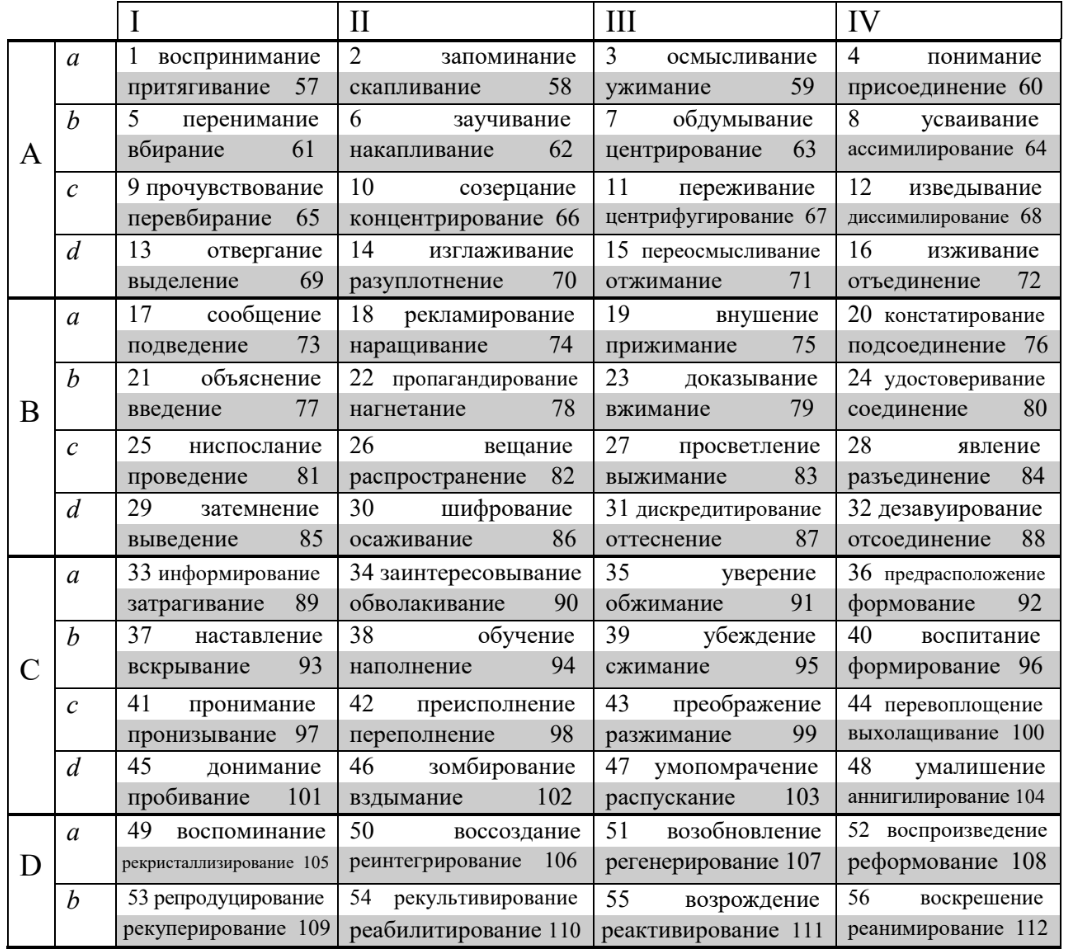
\includegraphics{figures/sd_actions/macroproc_table.png}
        ~\\}
    \scnrelfrom{источник}{\cite{Hardzei2017}}
    \scntext{explanation}{На изображении представлена типология \textit{воздействий}. Любое воздействие характеризуется принадлежностью четырём классам, соответствующим признакам классификации. Заштрихованы \textit{физические воздействия}.}
    \scnheader{Специфицируемые классы воздействий}
    \scnsuperset{\begin{scnset}
            \item формование
            ~\\\begin{scnreltoset}{пересечение}
                \scnitem{воздействие трансформации}
                \scnitem{воздействие среда-оболочка}
                \scnitem{воздействие генерации}
                \scnitem{физическое воздействие}
            \end{scnreltoset}
            \item притягивание
            ~\\\begin{scnreltoset}{пересечение}
                \scnitem{воздействие активизации}
                \scnitem{воздействие среда-оболочка}
                \scnitem{воздействие инициации}
                \scnitem{физическое воздействие}
            \end{scnreltoset}
            \item выхолащивание
            ~\\\begin{scnreltoset}{пересечение}
                \scnitem{воздействие трансформации}
                \scnitem{воздействие ядро-оболочка}
                \scnitem{воздействие генерации}
                \scnitem{физическое воздействие}
            \end{scnreltoset}
            \item аннигилирование
            ~\\\begin{scnreltoset}{пересечение}
                \scnitem{воздействие трансформации}
                \scnitem{воздействие оболочка-среда}
                \scnitem{воздействие генерации}
                \scnitem{физическое воздействие}
            \end{scnreltoset}
            \item введение
            ~\\\begin{scnreltoset}{пересечение}
                \scnitem{воздействие эксплуатации}
                \scnitem{воздействие оболочка-ядро}
                \scnitem{воздействие инициации}
                \scnitem{физическое воздействие}
            \end{scnreltoset}
            \item распускание
            ~\\\begin{scnreltoset}{пересечение}
                \scnitem{воздействие трансформации}
                \scnitem{воздействие оболочка-среда}
                \scnitem{воздействие амплификации}
                \scnitem{физическое воздействие}
            \end{scnreltoset}
            \item разжимание
            ~\\\begin{scnreltoset}{пересечение}
                \scnitem{воздействие трансформации}
                \scnitem{воздействие ядро-оболочка}
                \scnitem{воздействие амплификации}
                \scnitem{физическое воздействие}
            \end{scnreltoset}
            \item разъединение
            ~\\\begin{scnreltoset}{пересечение}
                \scnitem{воздействие эксплуатации}
                \scnitem{воздействие ядро-оболочка}
                \scnitem{воздействие генерации}
                \scnitem{физическое воздействие}
            \end{scnreltoset}
        \end{scnset}
    }
    \scnheader{Пример sc.g-текста, описывающего спецификацию воздействия}
    \scneq{\scnfileimage[20em]{figures/sd_actions/tapaz_description_example.png}}
    \scniselement{sc.g-текст}
    \scntext{explanation}{Представленный фрагмент базы знаний содержит декомпозицию воздействия во времени, указание принадлежности данного декомпозируемого воздействия и полученных в результате данной декомпозиции воздействий определенному их классу из приведенной выше классификации, а также указание участников данных акций.}
    \scntext{explanation}{Представленный фрагмент базы знаний можно протранслировать в следующий текст естественного языка: <<Некто принимает молоко, затем окисляет молоко, а именно: нормализует молоко до 15-процентной жирности, затем очищает молоко, затем пастеризует молоко, затем охлаждает молоко до определённой температуры, затем вносит закваску в молоко, затем сквашивает молоко, затем режет сгусток, затем подогревает сгусток, затем обрабатывает сгусток, затем отделяет сыворотку, затем охлаждает сгусток и, в итоге, производит творог>>.}
    \scnheader{субъект}
    \scnidtftext{часто используемый sc-идентификатор}{индивид}
    \scnidtf{активная сущность}
    \scnidtf{сущность, способная самостоятельно выполнять некоторые виды действий}
    \scnidtf{агент деятельности}
    \scnsuperset{Собственное Я}
    \scnsuperset{внутренний субъект ostis-системы}
    \scnsuperset{внешний субъект ostis-системы, с которым осуществляется взаимодействие}
    \scnsuperset{внешний субъект ostis-системы, с которым взаимодействие не происходит}
    \scnheader{внутренний субъект ostis-системы}
    \scnidtf{субъект, входящий в состав той \textit{ostis-системы, в базе знаний} которой он описывается}
    \scnsuperset{sc-агент}
    \scntext{explanation}{Под \textit{внутренним субъектом ostis-системы} понимается такой \textit{субъект}, который выполняет некоторые \textit{действия} в \uline{той же памяти}, в которой хранится его знак.
        ~\\К числу \textit{внутренних субъектов ostis-системы} относятся входящие в нее \textit{sc-агенты}, частные sc-машины, целые интеллектуальные подсистемы.}
    \scnheader{внешний субъект ostis-системы, с которым осуществляется взаимодействие}
    \scntext{explanation}{К числу \textit{внешних субъектов ostis-системы, с которыми осуществляется взаимодействие}, относятся конечные пользователи \textit{ostis-системы}, ее разработчики, а также другие компьютерные системы(причем не только интеллектуальные).}
    \scnheader{субъект действия\scnrolesign}
    \scnsubset{субъект\scnrolesign}
    \scnidtf{сущность, воздействующая на некоторую другую сущность в процессе заданного действия\scnrolesign}
    \scnidtf{сущность, создающая \textit{причину} изменений другой сущности (объекта действия)\scnrolesign}
    \scnidtf{быть субъектом данного действия\scnrolesign}
    \scnsuperset{субъект неосознанного воздействия\scnrolesign}
    \scnsuperset{субъект осознанного воздействия\scnrolesign}
    \scnidtf{субъект целенаправленного, активного воздействия\scnrolesign}
    \scnheader{исполнитель*}
    \scntext{explanation}{Связки отношения \textit{исполнитель*} связывают \textit{sc-элементы}, обозначающие \textit{действие} и \textit{sc-элементы}, обозначающие \textit{субъекта}, который предположительно будет осуществлять, осуществляет или осуществлял выполнение указанного \textit{действия}. Данное отношение может быть использовано при назначении конкретного исполнителя для проектной задачи по развитию баз знаний.В случае, когда заранее неизвестно, какой именно \textit{субъект*} будет исполнителем данного \textit{действия}, отношение \textit{исполнитель*} может отсутствовать в первоначальной формулировке \textit{задачи} и добавляться позже, уже непосредственно при исполнении.Когда действие выполняется (является \textit{настоящей сущностью}) или уже выполнено (является \textit{прошлой сущностью}), то исполнитель этого действия в каждый момент времени уже определён. Но когда действие только инициировано, тогда важно знать:
        \begin{enumerate}
            \item кто \uline{хочет} выполнить это действие и насколько важно для него стать исполнителем данного действия;
            \item кто \uline{может} выполнить данное действие и каков уровень его квалификации и опыта;
            \item кто и кому поручает выполнить это действие и каков уровень ответственности за невыполнение (приказ, заказ, официальный договор, просьба...)
        \end{enumerate}
        При этом следует помнить, что связь отношения \textit{исполнитель*} в данном случае также является временной прогнозируемой сущностью.Первым компонентом связок отношений \textit{исполнитель*} является знак \textit{действия}, вторым -- знак \textit{субъекта} исполнителя}
    \scnheader{объект воздействия\scnrolesign}
    \scnsubset{объект\scnrolesign}
    \scnidtf{сущность, на которую осуществляется воздействие в рамках заданного действия\scnrolesign}
    \scnidtf{сущность, являющаяся в рамках заданного действия исходным условием (аргументом), необходимым для выполнения этого действия\scnrolesign}
    \scntext{note}{Для разных действий количество объектов действий может быть различным.}
    \scntext{note}{Поскольку действие является процессом и, соответственно, представляет собой \textit{динамическую структуру}, то и знак \textit{субъекта действия\scnrolesign}, и знак \textit{объекта действия\scnrolesign} являются элементами данной структуры. В связи с этим можно рассматривать отношения \textit{субъект действия\scnrolesign} и \textit{объект действия\scnrolesign} как \textit{ролевые отношения}. Данный факт не  запрещает вводить аналогичные \textit{неролевые отношения}, однако это нецелесообразно.}
    \scnheader{продукт\scnrolesign}
    \scnidtf{быть продуктом заданного действия\scnrolesign}
    \scnsubset{продукт*}
    \scnsubset{результат*}
    \scnidtf{сухой остаток\scnrolesign}
    \scnidtf{то, ради чего может быть выполнено, выполняется или будет выполняться заданное действие\scnrolesign}
    \scntext{note}{Продуктом действия может быть некоторая материальная сущность, некоторое множество (тираж) одинаковых материальных сущностей, некоторая информационная конструкция}
    \scnheader{результат*}
    \scntext{explanation}{Связки отношения \textit{результат*} связывают \textit{sc-элемент}, обозначающий \textit{действие}, и \textit{sc-конструкцию}, описывающую результат выполнения рассматриваемого действия, другими словами, цель, которая должна быть достигнута при выполнении \textit{действия}.Результат может специфицироваться как атомарным высказыванием, так и неатомарным, т.е. конъюнктивным, дизъюнктивным, строго дизъюнктивным и т.д.В случае, когда успешное выполнение \textit{действия} приводит к изменению какой-либо конструкции в \textit{\mbox{sc-памяти}}, которое необходимо занести в историю изменений базы знаний или использовать для демонстрации протокола решении задачи, генерируется соответствующая связка отношения \textit{результат*}, связывающая задачу и \textit{sc-конструкцию}, описывающую данное изменение. Конкретный вид указанной \textit{\mbox{sc-конструкции}} зависит от типа действия.}
    \scnrelboth{следует отличать}{цель*}
    \scnidtf{спецификация планируемого результата*}
    \scntext{note}{Следует также отмечать то, что является непосредственно результатом (продуктом) некоторого действия, и то, что является предварительной (исходной, стартовой) спецификацией этого  результата. Далеко не всегда результатом действия является именно то, что планировалось (было целью) изначально.}
    \scnheader{класс выполняемых действий*}
    \scnidtf{класс действий, выполняемых классом субъектов*}
    \scntext{explanation}{Связки отношения \textit{класс выполняемых действий*} связывают классы \textit{субъектов} и классы действий, при этом предполагается, что каждый субъект указанного класса способен выполнять действия указанного класса действий.}
    \scnheader{заказчик*}
    \scntext{explanation}{Связки отношения \textit{заказчик*} связывают классы \textit{sc-элементы}, обозначающие \textit{действие}, и \textit{sc-элементы}, обозначающие  \textit{субъекта}, который заинтересован в выполнении данного действия и, как правило, инициирует его выполнение. Данное отношение может быть использовано при указании того, кто поставил проектную задачу по развитию баз знаний.Первым компонентов связок отношения \textit{заказчик*} является знак \textit{действия}, вторым -- знак \textit{субъекта}.}
    \scnheader{инициатор*}
    \scntext{explanation}{Связки отношения \textit{инициатор*} связывают \textit{sc-элемент}, обозначающий \textit{инициированное действие}, и знак \textit{субъекта}, который является инициатором данного \textit{действия}, то есть \textit{субъектом}, который инициировал данное \textit{действие} и, как правило, заинтересован в его успешном выполнении.}
    \scnheader{объект\scnrolesign}
    \scnidtf{аргумент действия\scnrolesign}
    \scntext{explanation}{Связки отношения \textit{объект\scnrolesign} связывают \textit{sc-элемент}, обозначающий \textit{действие}, и знак той сущности, над которой (по отношению к которой) осуществляется данное \textit{действие}, и, например, знак \textit{структуры}, подлежащий верификации.}
    \scnsuperset{первый аргумент действия\scnrolesign}
    \scnsuperset{второй аргумент действия\scnrolesign}
    \scnsuperset{третий аргумент действия\scnrolesign}
    \scnheader{класс аргументов*}
    \scnidtf{класс аргументов класса команд*}
    \scnidtf{быть классом sc-элементов, экземпляры которого являются аргументами для заданного класса команд*}
    \scnsuperset{класс первых аргументов*}
    \scnsuperset{класс вторых аргументов*}
    \scntext{explanation}{Связки отношения \textit{класс аргументов*} связывают \textit{классы команд} (подмножества множества \textit{команд}) и классы \textit{sc-элементов}, которые могут быть аргументами действий, соответствующих данному  \textit{классу команд}. В случае, когда  \textit{команды} данного класса имеют один аргумент, используется собственно отношение  \textit{класс аргументов*}, в случае, когда команды данного класса имеют более одного аргумента, то используются подмножества данного отношения, такие как \textit{класс первых аргументов*}, \textit{класс вторых аргументов*} и т.д.Если для некоторого \textit{класса команд} не указан тип какого-либо из аргументов, то предполагается, что в качестве данного аргумента может выступать любой \textit{sc-элемент}.Первым компонентом связок отношения \textit{класс аргументов*} является знак \textit{класса команд}, вторым -- знак класса \textit{sc-элемента}, которые могут быть \textit{аргументами действий\scnrolesign}, соответствующих данному \textit{классу команд}.}
    \bigskip
\end{scnsubstruct}
\scnendsegmentcomment{Предметная область и онтология субъектно-объектных спецификаций воздействий}
